
%(BEGIN_QUESTION)
% Copyright 2010, Tony R. Kuphaldt, released under the Creative Commons Attribution License (v 1.0)
% This means you may do almost anything with this work of mine, so long as you give me proper credit

Suppose a voltmeter registers 9 volts between test points {\bf A} and {\bf D} in this series-parallel circuit:

$$\includegraphics[width=15.5cm]{i04476x01.eps}$$

Identify the likelihood of each specified fault for this circuit.  Consider each fault one at a time (i.e. no coincidental faults), determining whether or not each fault could independently account for {\it all} measurements and symptoms in this circuit.

% No blank lines allowed between lines of an \halign structure!
% I use comments (%) instead, so that TeX doesn't choke.

$$\vbox{\offinterlineskip
\halign{\strut
\vrule \quad\hfil # \ \hfil & 
\vrule \quad\hfil # \ \hfil & 
\vrule \quad\hfil # \ \hfil \vrule \cr
\noalign{\hrule}
%
% First row
{\bf Fault} & {\bf Possible} & {\bf Impossible} \cr
%
\noalign{\hrule}
%
% Another row
$R_1$ failed open &  &  \cr
%
\noalign{\hrule}
%
% Another row
$R_2$ failed open &  &  \cr
%
\noalign{\hrule}
%
% Another row
$R_3$ failed open &  &  \cr
%
\noalign{\hrule}
%
% Another row
$R_4$ failed open &  &  \cr
%
\noalign{\hrule}
%
% Another row
$R_1$ failed shorted &  &  \cr
%
\noalign{\hrule}
%
% Another row
$R_2$ failed shorted &  &  \cr
%
\noalign{\hrule}
%
% Another row
$R_3$ failed shorted &  &  \cr
%
\noalign{\hrule}
%
% Another row
$R_4$ failed shorted &  &  \cr
%
\noalign{\hrule}
%
% Another row
Voltage source dead &  &  \cr
%
\noalign{\hrule}
} % End of \halign 
}$$ % End of \vbox

Finally, identify the {\it next} diagnostic test or measurement you would make on this system.  Explain how the result(s) of this next test or measurement help further identify the location and/or nature of the fault.

\vfil 

\underbar{file i04476}
\eject
%(END_QUESTION)





%(BEGIN_ANSWER)

This is a graded question -- no answers or hints given!

%(END_ANSWER)





%(BEGIN_NOTES)

A good problem-solving technique is to first determine how much voltage {\it should} exist between points A and D if the circuit is healthy.  Doing the series-parallel analysis on this circuit shows that 8 volts is normally dropped across resistor $R_1$, and thus there should be 8 volts between points A and D.

Since we know there are 9 volts there instead of 8, and we are only considering absolute faults (i.e. components failed completely shorted or completely open, no partial faults), we know it must be a fault capable of causing a relatively slight change in voltage.  In order to drop slightly more voltage across $R_1$ (there are no other components between points A and D but $R_1$), there must be slightly less resistance throughout the rest of the circuit: this suggests a shorted fault, but one that will not place full voltage across $R_1$.  There are only two possibilities left:

% No blank lines allowed between lines of an \halign structure!
% I use comments (%) instead, so that TeX doesn't choke.

$$\vbox{\offinterlineskip
\halign{\strut
\vrule \quad\hfil # \ \hfil & 
\vrule \quad\hfil # \ \hfil & 
\vrule \quad\hfil # \ \hfil \vrule \cr
\noalign{\hrule}
%
% First row
{\bf Fault} & {\bf Possible} & {\bf Impossible} \cr
%
\noalign{\hrule}
%
% Another row
$R_1$ failed open &  & $\surd$ \cr
%
\noalign{\hrule}
%
% Another row
$R_2$ failed open &  & $\surd$ \cr
%
\noalign{\hrule}
%
% Another row
$R_3$ failed open &  & $\surd$ \cr
%
\noalign{\hrule}
%
% Another row
$R_4$ failed open &  & $\surd$ \cr
%
\noalign{\hrule}
%
% Another row
$R_1$ failed shorted &  & $\surd$ \cr
%
\noalign{\hrule}
%
% Another row
$R_2$ failed shorted &  & $\surd$ \cr
%
\noalign{\hrule}
%
% Another row
$R_3$ failed shorted & $\surd$ &  \cr
%
\noalign{\hrule}
%
% Another row
$R_4$ failed shorted & $\surd$ &  \cr
%
\noalign{\hrule}
%
% Another row
Voltage source dead &  & $\surd$ \cr
%
\noalign{\hrule}
} % End of \halign 
}$$ % End of \vbox

Sure enough, if we re-calculate the voltage drop between points A and D with only 500 ohms in the D-F-E branch of the circuit, we get 9 volts between A and D.

\vskip 10pt

For a next test to determine which is the failed-shorted resistor ($R_3$ or $R_4$), we may measure voltage across either one.  The one with zero voltage across it is the shorted resistor.  The one with 3 volts across it is the functioning resistor.

%INDEX% Troubleshooting review: electric circuits

%(END_NOTES)

